% !TeX spellcheck = de_DE
\documentclass{alex_gp}

\name{Alexander Helbok}
\course{Grundpraktikum}
\hwnumber{2}
\spacing{}

\setlength{\columnsep}{1cm}
\begin{document}
\renewcommand{\labelenumi}{\alph{enumi})}

\begin{mybox}{Kalibrierung des Rades}
	Das Messgerät wurde von Tischkante bis zur Wand geschoben und hat währenddessen die Distanz aufgezeichnet. Die zurückgelegte Strecke setzt sich aus dem Abstand zwischen Wand und Tischkante minus der Länge des IOLabs \footnote{https://www.macmillanlearning.com/college/us/digital/iolab/technical-specs} zusammen und wurde auf \( d = 0.665(1) \unit{m} \) gemessen. Die Länge des Tisches wurde an der Kante gemessen, wo man unter Annahme eines rechtwinkeligen Tisches das Lineal äußerst gerade halten kann. Deshalb wurde diese Fehlerquelle nicht miteinbezogen, da sie vernachlässigbar klein ist im Vergleich zum Ablesefehler.\par 
	Der Fehler der Distanzmessung des IOLabs wird bei \( 1 \unit{mm} \) angenommen
	
	\begin{minipage}{0.35\textwidth}
		\begin{tabular}{@{} rr @{}}\toprule
			s [m] & a \\ \midrule
			0.661(1) & 0.994(2) \\
			0.663(1) & 0.997(2) \\
			0.663(1) & 0.997(2) \\
			0.664(1) & 0.998(2) \\
			0.662(1) & 0.995(2) \\
			0.662(1) & 0.995(2) \\
			0.661(1) & 0.994(2) \\
			0.660(1) & 0.992(2) \\
			0.664(1) & 0.998(2) \\
			0.665(1) & 1.000(2) \\
			\bottomrule
		\end{tabular}
		\captionof{table}{Gemessene zurückgelegte Strecke \( s \) und die dazugehörige Proportionalitätskostante \( a \)}
		\label{table:1}
	\end{minipage}
\end{mybox}

\begin{mybox}{Bemessung von \( g \)}
	Um die Erdbeschleunigung \( g \) zu messen, wurde ein Pendel mit einem Kraftsensor ausgestattet. Die Länge \( L \) des Pendels setzt sich aus der Fadenlänge, an welchem das IOLab befestigt ist, und der Distanz zwischen Aufhängepunkt am Messgerät zu dessen Massezentrum zusammen, welchen mit einem \( 4\times 4 \unit{mm} \) Kasten markiert ist. Letztere Distanz wurde mit einer elektronischen Schublehre von der Kante bis zum Mittelpunkt der Box gemessen; die prominente Unsicherheit kommt hier aus der wagen Kennzeichnung der Schwerpunkts und wurde auf \( 2 \unit{mm} \) geschätzt. Der Fehler der Fadenlänge beträgt auch \( 2 \unit{mm} \). Hierbei wurde der Ablesefehler, die Krümmung des Maßbandes und die Lokalisierung der Drehachse berücksichtigt. Die Gesamtlänge beträgt 
	\begin{equation}
		L = 0.538(3) \unit{m}
	\end{equation}
	Die Periodendauer \( T_0 \) des mathematische Pendels wird unter Annahme der Kleinwinkelnäherung durch 
	\begin{equation}\label{eqn:T0}
		T_0 = 2\pi\sqrt{\tfrac{L}{g}}
	\end{equation}
	beschrieben, wobei \( g \) die Gravitationsbeschleunigung auf der Erde darstellt. Um die Periodendauer mithilfe der Daten des Kraftsensors zu bestimmen wurde eine Sinuskurve der Form \( A * \sin(\omega x + \varphi) + k \) an die Messpunkte angepasst. Der Fitprozess verlief in drei Schritten.\par 
	Da die Daten sehr verrauscht waren mussten sie zuerst geglättet werden. Danach wurde ein Sinus in der allgemeinen Form mit vier freien Parametern an die Daten von \( t = 4 \unit{s} \) bis \( t = 5 \unit{s} \) angepasst. Im dritten Schritt wurde wieder ein Sinus mit zwei freien Variablen (\( \omega, \varphi \)) an den Zeitraum von zwei bis sieben Sekunden gefittet, wobei \( A \) und \( k \) auf den im zweiten Schritt ermittelten Werten festgehalten wurden. \par 
	Das Ergebnis ist in Abbildung \ref{fig:sine} dargestellt und liefert eine Periode von
	\begin{equation}\label{eqn:period}
		T_0 = 2 \frac{2\pi}{\omega} = 1.4955(3) \unit{s}
	\end{equation}
	Hier darf man den Faktor 2 nicht vergessen, der daher kommt, dass die Kraft auf den Sensor des Pendels bezüglich der Senkrechten symmetrisch ist und in einer Periode zwei Maxima (maximale Auslenkung) und zwei Minima (Ruhelage) durchlaufen werden.
	\begin{figure}[H]
		\vspace{-0.5cm}		
		\centering
		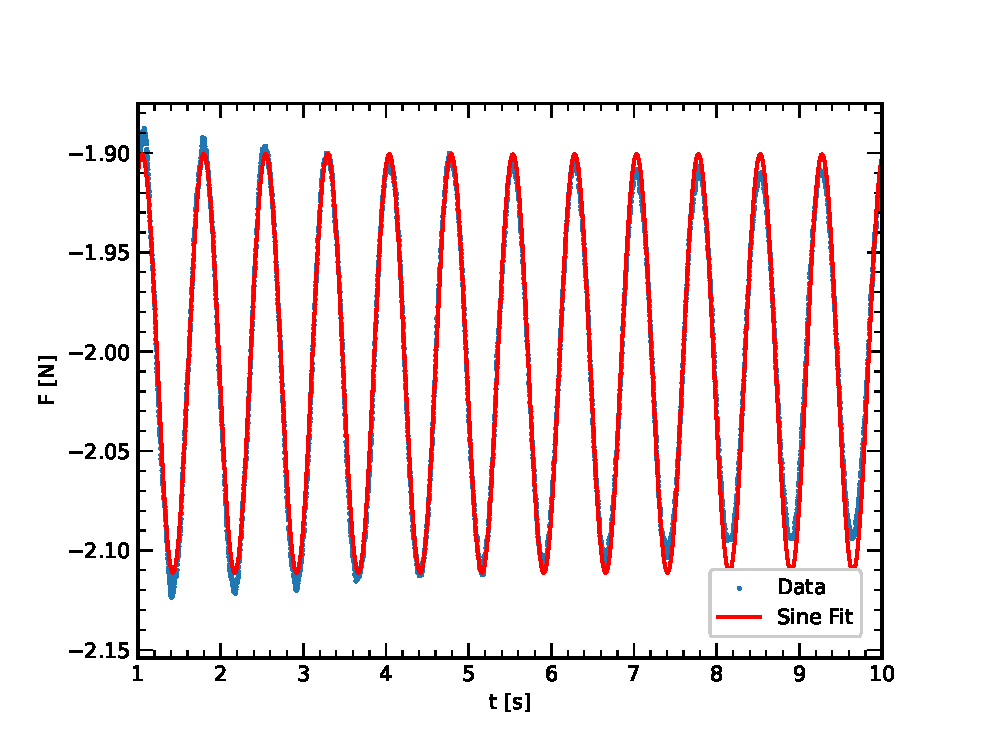
\includegraphics[width=\textwidth]{Versuch2_1.eps}
		\caption{Beschönigte Daten des Kraftsensors während der ersten 12 „schönen“ Schwingungen des Pendelvorgangs. Eine Sinuskurve wurde in den Zeitraum von 2 bis 7 Sekunden angepasst.}
		\label{fig:sine}
	\end{figure}
	Setzt man die ermittelten Werte in Gleichung \ref{eqn:T0} ein erhält man
	\begin{equation}\label{eqn:g0}
		g = 4\pi^2 \frac{L}{T_0^2} = 9.50(5) \unit{\a}
	\end{equation}
	Gleichung \ref{eqn:T0} macht Gebrauch der Kleinwinkelnäherung, Terme aus der Taylorentwicklung der genäherten Winkelfunktionen einbauen und erhält dann
	\begin{equation}\label{eqn:T2}
		T_2 = \left(1 + \tfrac{\theta_0^2}{16}\right) T_0 = 2\pi\left(1 + \tfrac{\theta_0^2}{16}\right)\sqrt{\tfrac{L}{g}}
	\end{equation}
	\( \theta_0 \) beschreibt hier die maximale Auslenkung des Pendels und kann mithilfe einer zweiten Messung in Ruhelage bestimmt werden. Die Kraft in Ruhelage beträgt \( F_0 = mg = -1.97095(1) \unit{N} \) und wurde als ungewichteter Mittelwert einer 30 Sekunden langen Messung berechnet. Die Kraft beim Winkel \( \theta_0 \) ist gerade \( F(\theta_0) = mg\cos(\theta_0) = -1.90069(6) \unit{N} \) und ist die Summe der Amplitude \( A \) und der Vertikalverschiebung \( k \) aus dem Sinusfit. \( \theta_0 \) lässt sich also wie folgt schreiben
	\begin{equation}\label{eqn:theta}
		\theta_0 = \arccos(\frac{F(\theta_0)}{F_0}) = \ang{15.344(7)}
	\end{equation}
	Jetzt kann man Werte in \ref{eqn:T2} einsetzen und erhält
	\begin{equation}\label{eqn:g1}
		g = 4\pi^2 \frac{L}{T_0^2}\frac{1}{\left(1 + \tfrac{\theta_0^2}{16}\right)} = 9.45(5) \unit{\a}
	\end{equation}
\end{mybox}

\begin{mybox}{Kalibrierung des Kraftsensors}
	\begin{vwcol}[widths={0.6,0.4}, sep=.8cm, justify=flush,rule=0pt, indent=1em] 
		Um die Präzision und Richtigkeit des Kraftsensors zu eruieren wurde eine Probemasse in Form von Münzen an den Sensor gehängt und den gemessen Wert mit dem Berechneten verglichen. Anzahl und Masse der verwendeten Münzen bitte Tabelle \ref{table:2} entnehmen.\par
		Es wurden für \( 10 \unit{s} \) Daten vom  Kraftsensor aufgezeichnet und davon der ungewichtete Mittelwert berechnet. Die gemessene Kraft 
		\begin{equation}
			F_{\text{gem}} = -0.394 \unit{N}
		\end{equation}
		wird mit drei signifikanten Stellen angegeben, um die des berechneten Werts zu matchen. Die Angabe der Kraft erfolgt hier ohne Fehler, weil der Standardfehler so gering ist (da in den \( 10 \unit{s} \) fast 30.000 Datenpunkte gesammelt wurden).
		\newpage
		\begin{minipage}{0.35\textwidth}
			\begin{tabular}{@{} rrr @{}}\toprule
				Wert & Anzahl & Masse [g] \\ \midrule
				1 Cent & 2 & 2.30(2) \\
				2 Cent & 7 & 3.06(3) \\
				5 Cent & 3 & 3.92(4) \\
				10 Cent & 1 & 4.10(4) \\
				\midrule
				\( \sum \) & 13 & 41.9(3) \\
				\bottomrule
			\end{tabular}
			\captionof{table}{Anzahl der verwendeten Münzen und deren Einzelgewicht.}
			\label{table:2}
		\end{minipage}
	\end{vwcol}
	
\end{mybox}


\end{document}